\documentclass[11pt]{article}
\usepackage[margin=1in]{geometry}
\usepackage{amsmath,amssymb}
\usepackage{enumitem}
\usepackage{tikz}
\usepackage{xcolor}
\usepackage{array}
\usepackage{fancyhdr}

% ---- solutions toggle: \newif set by the build script -----------------
\newif\ifsol
\input{soltoggle}

\definecolor{solblue}{HTML}{0B2B5C}
\definecolor{solgreen}{HTML}{0B5F55}

\pagestyle{fancy}
\fancyhf{}
\renewcommand{\headrulewidth}{0pt}
\cfoot{\thepage}

\setlength{\parindent}{0pt}
\setlength{\parskip}{6pt}

% ---- CS188-style masthead --------------------------------------------
\newcommand{\masthead}[3]{%
  \noindent\rule{\textwidth}{2pt}\\[2pt]
  \noindent
  \begin{minipage}[b]{0.45\textwidth}
    {\Large #1}\\{\Large #2}
  \end{minipage}
  \hfill
  \begin{minipage}[b]{0.5\textwidth}
    \raggedleft{\huge #3}
  \end{minipage}\\[4pt]
  \noindent\rule{\textwidth}{2pt}\\[-4pt]
}

% ---- answer space / solution block -----------------------------------
\newcommand{\ans}[1]{\ifsol\relax\else\vspace{#1}\filbreak\fi}

\newenvironment{solution}
  {\ifsol
     \par\vspace{4pt}\noindent
     \color{solgreen}\textbf{Solution.}\enspace\itshape\ignorespaces
   \else
     \setbox0\vbox\bgroup
   \fi}
  {\ifsol\par\normalcolor\upshape\vspace{4pt}\else\egroup\fi}

\newcommand{\qhead}[1]{\section*{#1}}

\newcommand{\bub}{$\bigcirc$~}

\begin{document}

\masthead{COMP 469}{Fall 2026}{Take-Home Discussion 2}

\vspace{6pt}
{\large\textbf{Chapter 2: Intelligent Agents}}\hfill Name(s):\enspace\rule{2.4in}{0.4pt}

\vspace{2pt}
Covers AIMA 4e \S2.1--\S2.4.7. \textbf{No search algorithm is needed anywhere in this
handout.} If you find yourself describing how to \emph{compute} a route, you have wandered
into the next chapter --- every question here is about what an agent perceives, what counts
as success, what kind of environment it faces, and which agent design that environment
demands. Work in groups of two or three. Answers are graded on reasoning, not length.

\ifsol
\vspace{2pt}
{\color{solblue}\textbf{INSTRUCTOR EDITION.} Solutions shown in green italics.}
\fi

% ======================================================================
\qhead{1\quad The Three-Square Vacuum World}

Extend the vacuum world of Figure~2.2 to three squares in a row, $A$, $B$, and $C$. Each
square is either Clean or Dirty. The agent perceives its own location and the status of
the square it occupies, so a percept looks like $[B,\textit{Dirty}]$. The available actions
are \textit{Left}, \textit{Right}, \textit{Suck}, and \textit{NoOp}. The agent starts in $A$.
Moving into a wall leaves the agent where it is. Sucking cleans the current square, and
clean squares stay clean.

\begin{center}
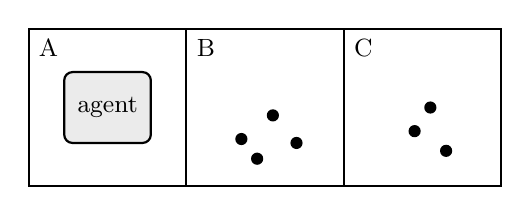
\begin{tikzpicture}[scale=1]
  \foreach \i/\lab in {0/A, 1/B, 2/C} {
    \draw[thick] (\i*2,0) rectangle (\i*2+2,2);
    \node at (\i*2+0.25,1.75) {\small \lab};
  }
  % dirt in B and C
  \foreach \p in {(2.7,0.6),(3.1,0.9),(2.9,0.35),(3.4,0.55)} \fill \p circle (2.2pt);
  \foreach \p in {(4.9,0.7),(5.3,0.45),(5.1,1.0)} \fill \p circle (2.2pt);
  % agent in A
  \draw[thick,fill=black!8,rounded corners=3pt] (0.45,0.55) rectangle (1.55,1.45);
  \node at (1.0,1.0) {\small agent};
\end{tikzpicture}
\end{center}

Unless a part says otherwise, the performance measure awards one point for each clean
square at each time step, over a lifetime of 1000 steps.

\begin{enumerate}[label=(\alph*),leftmargin=*]

\item How many distinct percepts are there? How many distinct percept sequences of length
exactly $t$? Write a closed-form expression for the number of rows a lookup table needs in
order to cover every percept sequence of length $1$ through $T$.
\ans{1.1in}
\begin{solution}
There are $3\times 2=6$ percepts, so $6^{t}$ sequences of length exactly $t$, and
\[
\sum_{t=1}^{T} 6^{t} \;=\; \frac{6^{\,T+1}-6}{5}
\]
rows in total.
\end{solution}

\item Tabulate the agent function for every percept sequence of length one. Fill in an
action that is rational under the performance measure above.

\begin{center}
\begin{tabular}{|l|c|}
\hline
\textbf{Percept sequence} & \textbf{Action} \\ \hline
$[A,\textit{Clean}]$  & \ifsol \textit{Right} \else \rule[-0.11in]{1.6in}{0pt}\rule[-0.11in]{0pt}{0.26in} \fi \\ \hline
$[A,\textit{Dirty}]$  & \ifsol \textit{Suck}  \else \rule[-0.11in]{1.6in}{0pt}\rule[-0.11in]{0pt}{0.26in} \fi \\ \hline
$[B,\textit{Clean}]$  & \ifsol \textit{Right} \else \rule[-0.11in]{1.6in}{0pt}\rule[-0.11in]{0pt}{0.26in} \fi \\ \hline
$[B,\textit{Dirty}]$  & \ifsol \textit{Suck}  \else \rule[-0.11in]{1.6in}{0pt}\rule[-0.11in]{0pt}{0.26in} \fi \\ \hline
$[C,\textit{Clean}]$  & \ifsol \textit{Left}  \else \rule[-0.11in]{1.6in}{0pt}\rule[-0.11in]{0pt}{0.26in} \fi \\ \hline
$[C,\textit{Dirty}]$  & \ifsol \textit{Suck}  \else \rule[-0.11in]{1.6in}{0pt}\rule[-0.11in]{0pt}{0.26in} \fi \\ \hline
\end{tabular}
\end{center}
\begin{solution}
Suck whenever the current square is dirty; otherwise move toward a square the agent has
not just cleaned. At $B$, either \textit{Left} or \textit{Right} is defensible --- movement
is free and the agent has no evidence favoring one side --- as long as the choice is
stated. At $C$, only \textit{Left} makes progress, since \textit{Right} runs into the wall.
\end{solution}

\item Write a simple reflex agent program, in at most six lines of pseudocode, that
produces exactly the table you filled in for part (b). Then evaluate your expression from
part (a) at $T=10$ and compare the two numbers. State in one sentence what the comparison
is meant to show.
\ans{1.6in}
\begin{solution}
\begin{tabbing}
\quad\=\textbf{function} \textsc{Reflex-Vacuum}$([\textit{location},\textit{status}])$ \textbf{returns} an action\\
\>\quad \textbf{if} \textit{status} $=$ \textit{Dirty} \textbf{then return} \textit{Suck}\\
\>\quad \textbf{else if} \textit{location} $= C$ \textbf{then return} \textit{Left}\\
\>\quad \textbf{else return} \textit{Right}
\end{tabbing}
At $T=10$ the table needs $(6^{11}-6)/5 = 72{,}559{,}410$ rows, roughly $7.3\times10^{7}$,
against four lines of program. The table is an external description of the behavior; the
program is what we actually build, and it is small because it exploits a regularity in the
environment --- the right action for a dirty square is the same no matter what came before.
\end{solution}

\item Now change the performance measure so that each movement costs one point, while
\textit{Suck} and \textit{NoOp} are free. Is your agent from part (c) still rational? If
not, say what behavior becomes rational once the floor is entirely clean, and name the
action that makes it possible.
\ans{1.2in}
\begin{solution}
No. Once all three squares are clean the agent keeps shuttling between them and loses a
point per step for the rest of its 1000-step lifetime. The rational behavior is to stop,
which requires \textit{NoOp}. Nothing about the program changed --- only the performance
measure did. Rationality is a relation among the performance measure, the prior knowledge,
the action set, and the percept sequence, not a property of the code.
\end{solution}

\item Your part (c) agent cannot actually tell when the floor is clean, because its action
depends only on the current percept. What is the smallest capability you must add, what is
the name Chapter~2 gives the resulting design, and which two models does that design
maintain?
\ans{1.2in}
\begin{solution}
Add internal state: a record of which squares have been observed clean since they were last
visited (plus the agent's own location if it must be tracked). That is a \textbf{model-based
reflex agent}. It maintains a \textbf{transition model} --- how the world changes on its own
and in response to the agent's actions --- and a \textbf{sensor model} --- what the percepts
say about the world state.
\end{solution}

\item Suppose the location sensor fails, so the percept is now just \textit{Clean} or
\textit{Dirty}. Explain why no simple reflex agent with a deterministic rule set can be
rational here. What partial fix does the chapter offer, and why does it call it only a
trick rather than a solution?
\ans{1.4in}
\begin{solution}
The percept \textit{Clean} now occurs at $A$, $B$, and $C$, and those three situations call
for different actions, but a deterministic reflex agent must return the same action for the
same percept. A rule that always moves \textit{Right} on \textit{Clean} gets stuck against
the wall at $C$; one that always moves \textit{Left} gets stuck at $A$. Randomizing the
choice will eventually escape the loop and, in a world this small, do reasonably well. The
chapter treats randomization as a useful trick rather than a general answer: it escapes
loops without supplying any knowledge, and in larger or safety-critical tasks random action
is inefficient or dangerous. The real fix is internal state.
\end{solution}

\end{enumerate}

\newpage
% ======================================================================
\qhead{2\quad PEAS and Two Task Environments}

Consider two systems.

\begin{itemize}[leftmargin=*,itemsep=2pt]
\item \textbf{Agent I} --- a tournament chess program playing under a game clock.
\item \textbf{Agent II} --- an autonomous hospital delivery robot that carries supplies
between wards along corridors it shares with people, gurneys, and cleaning carts.
\end{itemize}

\begin{enumerate}[label=(\alph*),leftmargin=*]

\item Write a PEAS description for Agent II with at least two concrete items in each
category. ``Be helpful'' and ``do a good job'' are not performance measures.

\begin{center}
\begin{tabular}{|>{\raggedright\arraybackslash}p{1.15in}|>{\raggedright\arraybackslash}p{4.6in}|}
\hline
\textbf{Performance} & \ifsol \textit{Deliveries completed on time; zero collisions with people or equipment; correct item delivered to the correct ward; battery managed so the robot is never stranded; low corridor obstruction time.} \else \rule[-0.62in]{0pt}{0.14in} \fi \\ \hline
\textbf{Environment} & \ifsol \textit{Corridors, elevators, doorways, ward layouts, pedestrians and staff, gurneys and carts, spills and closed doors, delivery requests, shift schedules.} \else \rule[-0.62in]{0pt}{0.14in} \fi \\ \hline
\textbf{Actuators} & \ifsol \textit{Drive wheels, steering or differential drive, brakes, cargo compartment latch, elevator call signal, warning tone and status display.} \else \rule[-0.62in]{0pt}{0.14in} \fi \\ \hline
\textbf{Sensors} & \ifsol \textit{Lidar or depth camera, bump and proximity sensors, wheel odometry, floor map and localization, cargo-bay sensor, battery gauge, network feed of delivery requests.} \else \rule[-0.62in]{0pt}{0.14in} \fi \\ \hline
\end{tabular}
\end{center}

\item Classify both agents on the seven dimensions of \S2.3.2. One or two words per cell.

\begin{center}
\begin{tabular}{|>{\raggedright\arraybackslash}p{2.05in}|>{\raggedright\arraybackslash}p{1.85in}|>{\raggedright\arraybackslash}p{1.85in}|}
\hline
\textbf{Dimension} & \textbf{I: chess with a clock} & \textbf{II: hospital robot} \\ \hline
Observable & \ifsol \textit{Fully} \else \rule[-0.20in]{0pt}{0.14in} \fi & \ifsol \textit{Partially} \else \fi \\ \hline
Agents & \ifsol \textit{Multiagent, competitive} \else \rule[-0.20in]{0pt}{0.14in} \fi & \ifsol \textit{Multiagent, mostly cooperative} \else \fi \\ \hline
Determinism & \ifsol \textit{Deterministic} \else \rule[-0.20in]{0pt}{0.14in} \fi & \ifsol \textit{Nondeterministic} \else \fi \\ \hline
Episodes & \ifsol \textit{Sequential} \else \rule[-0.20in]{0pt}{0.14in} \fi & \ifsol \textit{Sequential} \else \fi \\ \hline
Time & \ifsol \textit{Semidynamic} \else \rule[-0.20in]{0pt}{0.14in} \fi & \ifsol \textit{Dynamic} \else \fi \\ \hline
State / action & \ifsol \textit{Discrete} \else \rule[-0.20in]{0pt}{0.14in} \fi & \ifsol \textit{Continuous} \else \fi \\ \hline
Knowledge & \ifsol \textit{Known} \else \rule[-0.20in]{0pt}{0.14in} \fi & \ifsol \textit{Partly unknown} \else \fi \\ \hline
\end{tabular}
\end{center}
\begin{solution}
Chess is fully observable and known: both players see the whole board and the rules are
given in advance. It is deterministic --- a legal move has exactly one outcome --- even
though the opponent's \emph{choice} is uncertain, which is a multiagent property, not a
determinism property. Getting this distinction right is the point of the row.
\end{solution}

\item Students most often miss the \textbf{Time} row. Explain why chess with a clock is
semidynamic rather than static, and name a task environment from \S2.3.2 that is simply
static.
\ans{0.9in}
\begin{solution}
The board does not change while a player deliberates, so the environment itself is static;
but the clock runs, so the agent's performance score changes with deliberation time. That
combination is exactly what \emph{semidynamic} means. A crossword puzzle is static: neither
the world nor the score moves while you think.
\end{solution}

\item \emph{Known} and \emph{observable} are independent. For the hospital robot, describe
(i) a situation in which its environment is known but only partially observable, and
(ii) a change that would make some part of it unknown while it remains fully observable.
\ans{1.2in}
\begin{solution}
(i) The floor plan, the rules of motion, and the elevator's behavior are all known in
advance, yet the robot cannot see a gurney parked around the next corner --- known,
partially observable.
(ii) Install a new automated door whose signalling protocol the robot has never used. A
ceiling camera may show the robot the entire corridor, so the state is fully observable,
but the effect of its own ``open door'' action is not yet known --- fully observable,
unknown. Known/unknown is about the designer's and agent's grip on the \emph{rules}, not
about what the sensors can see.
\end{solution}

\item The chapter separates \emph{nondeterministic} from \emph{stochastic}. Which label
applies to the robot's model of a pedestrian stepping into its path, and what would have to
change for the other label to apply?
\ans{0.9in}
\begin{solution}
As stated, nondeterministic: the model lists possible outcomes --- the pedestrian steps
left, steps right, or stops --- without quantifying them. It becomes stochastic only when
the model attaches probabilities, for example a 15\% chance of stepping into the path. Both
mean the next state is not determined by the current state and action; only stochastic
models commit to numbers.
\end{solution}

\item A vendor proposes the performance measure ``minimize average delivery time.'' Give one
concrete way a perfectly rational agent could maximize this measure while producing
behavior the hospital would reject. Rewrite the measure to close the loophole, and name the
problem from Chapter~1 that this illustrates.
\ans{1.4in}
\begin{solution}
Any answer that optimizes the stated number rather than the intended outcome. Examples: the
robot serves only nearby wards and lets distant requests sit in the queue forever, so the
average over \emph{completed} deliveries looks excellent; or it drives fast through crowded
corridors, trading safety for speed the measure never scores. A repaired measure scores the
state of the world we actually want: on-time completion rate across \emph{all} requests
including the slowest, zero collisions and near-misses, correct item and ward, and a cap on
worst-case wait rather than an average. This is the King Midas problem, or value alignment
--- a capable optimizer faithfully maximizing a badly specified objective. Note also that
an average conceals variance: two robots with the same average delivery time can behave very
differently, and if variance matters the measure has to say so.
\end{solution}

\end{enumerate}

\newpage
% ======================================================================
\qhead{3\quad Agent Designs, Rationality, and Representation}

\begin{enumerate}[label=(\alph*),leftmargin=*]

\item For each system below, select the \textbf{least complex} agent design from Chapter~2
that is adequate for the task as described. Choose exactly one bubble per row.

\newcommand{\optbub}[2]{\ifsol\ifnum#1=#2$\bullet$\else$\bigcirc$\fi\else$\bigcirc$\fi}
\newcommand{\designrow}[6]{%
  #1 \\[1pt]
  {\small
  \hspace*{0.6em}
  \makebox[1.28in][l]{\optbub{#6}{1}~simple reflex}
  \makebox[1.62in][l]{\optbub{#6}{2}~model-based reflex}
  \makebox[1.08in][l]{\optbub{#6}{3}~goal-based}
  \makebox[1.16in][l]{\optbub{#6}{4}~utility-based}
  \makebox[0.85in][l]{\optbub{#6}{5}~learning}}
  \\[7pt]}

\begin{enumerate}[label=(\roman*),leftmargin=1.2em]
\item[] \designrow{(i)~~A smoke alarm that sounds whenever particulate density crosses a fixed threshold.}{}{}{}{}{1}
\item[] \designrow{(ii)~~A floor-cleaning robot whose sensors cannot tell which room it is in, but which must cover every room.}{}{}{}{}{2}
\item[] \designrow{(iii)~~A delivery drone that must reach a specified address; any route that arrives is equally acceptable.}{}{}{}{}{3}
\item[] \designrow{(iv)~~A router that must weigh a faster arrival against a higher chance of missing a pickup window.}{}{}{}{}{4}
\item[] \designrow{(v)~~A mail filter deployed at an organization whose spam patterns were not known at design time.}{}{}{}{}{5}
\end{enumerate}

\begin{solution}
(i) The correct action is a function of the current percept alone. (ii) Coverage requires
remembering where it has been, and the percept does not supply that --- partial
observability calls for internal state. (iii) A binary goal test is enough because all
successful outcomes are equally good. (iv) Two outcomes both satisfy the goal but differ in
quality and carry uncertainty, which is exactly what a utility function is for.
(v) The relevant regularities are unknown at design time, so the agent has to improve its
own components from feedback. Note that (v) is not exclusive with the others: a learning
agent is built \emph{on top of} one of the first four designs.
\end{solution}

\item True or false, with a one-line justification for each.

\begin{enumerate}[label=(\roman*),leftmargin=1.2em,itemsep=4pt]
\item An agent that chose a rational action and then suffered the worst possible outcome
acted irrationally. \ifsol{\color{solgreen}\textbf{~F}}\fi
\item A rational agent never has reason to take an action whose only payoff is information.
\ifsol{\color{solgreen}\textbf{~F}}\fi
\item Whether an agent is rational can be determined by inspecting its program.
\ifsol{\color{solgreen}\textbf{~F}}\fi
\item An agent that relies entirely on its designer's prior knowledge lacks autonomy.
\ifsol{\color{solgreen}\textbf{~T}}\fi
\end{enumerate}
\ans{1.1in}
\begin{solution}
(i) False. Rationality maximizes \emph{expected} performance given the evidence available at
the time; perfection would maximize actual performance, and demanding it would require a
crystal ball. (ii) False. Information gathering is rational whenever better percepts improve
later decisions --- looking both ways before crossing does not move you across the street,
and is still the right action. (iii) False. Rationality is a relation among the performance
measure, prior knowledge, action set, and percept sequence; the same four lines of code are
rational under one specification and irrational under another. (iv) True. That is what the
dung beetle and the sphex wasp illustrate: behavior that is rational only in the exact
environment their built-in assumptions describe, and that degrades to nonsense the moment
the assumption is violated.
\end{solution}

\item A table-driven agent stores one entry per percept sequence. Let $|P|$ be the number of
distinct percepts and $T$ the agent's lifetime in steps. Write the number of table entries,
then give the \textbf{three independent} reasons the chapter says this design fails, and name
the analogy it offers for what should replace the table.
\ans{1.3in}
\begin{solution}
The table needs $\sum_{t=1}^{T}|P|^{t}$ entries. The three failures are independent: no
physical agent has room to \emph{store} the table; no designer has time to \emph{build} it;
and no agent could ever have enough experience to \emph{learn} all the right entries. The
design is not incorrect --- filled in properly it implements exactly the agent function we
want --- it is simply unbuildable. The analogy is the replacement of large printed
square-root tables by Newton's method: a short program that captures the structure which
generated the table. The chapter's wager is that the same can be done for intelligent
behavior in general.
\end{solution}

\item Match each learning-agent component to its job, then answer the follow-up.

\begin{center}
\begin{tabular}{|>{\raggedright\arraybackslash}p{1.5in}|>{\raggedright\arraybackslash}p{4.3in}|}
\hline
Performance element & \ifsol \textit{Selects the external action --- everything we previously called ``the agent.''} \else \rule[-0.19in]{0pt}{0.14in} \fi \\ \hline
Critic & \ifsol \textit{Judges how the agent is doing against a fixed external performance standard.} \else \rule[-0.19in]{0pt}{0.14in} \fi \\ \hline
Learning element & \ifsol \textit{Uses the critic's feedback to modify the performance element's components.} \else \rule[-0.19in]{0pt}{0.14in} \fi \\ \hline
Problem generator & \ifsol \textit{Proposes actions that look suboptimal now but produce informative experience.} \else \rule[-0.19in]{0pt}{0.14in} \fi \\ \hline
\end{tabular}
\end{center}

Follow-up: why must the performance standard be fixed and sit conceptually \emph{outside}
the agent?
\ans{0.85in}
\begin{solution}
Percepts carry no verdict on their own --- a chess program can perceive that it has
delivered checkmate and still need a standard to know that this is good news. If the agent
could edit that standard, it could always succeed by lowering the bar: redefining success
instead of improving behavior. This is the slide to point back to when reward hacking comes
up later in the course.
\end{solution}

\item Return to the three-square vacuum of Question~1. Write the state ``the agent is in $B$,
$A$ is clean, $B$ is dirty, $C$ is clean'' in each of the three representations.
\ans{1.4in}
\begin{solution}
\textbf{Atomic:} one indivisible label such as $s_{17}$, with no internal parts the agent can
inspect. \textbf{Factored:} a fixed set of variables with values, e.g.\
$\textit{loc}=B$, $\textit{dirtA}=\text{false}$, $\textit{dirtB}=\text{true}$,
$\textit{dirtC}=\text{false}$. \textbf{Structured:} objects and relations, e.g.\
$\textit{At}(\textit{agent},B)$, $\textit{Dirty}(B)$, $\textit{RightOf}(B,A)$,
$\textit{RightOf}(C,B)$.
\end{solution}

\item Which of the three representations is required to express ``every square to the left of
the agent is clean'' without enumerating the cases one by one, and what does the chapter say
you pay for that expressiveness?
\ans{0.85in}
\begin{solution}
Structured. The claim quantifies over objects and depends on a relation between them, which
neither an atomic label nor a fixed list of variables can state in general --- a factored
representation can only enumerate the specific combinations. The price is that reasoning
becomes computationally harder as the representation becomes more expressive; the chapter
presents atomic $\rightarrow$ factored $\rightarrow$ structured as an axis of increasing
expressiveness with increasing cost.
\end{solution}

\item Is a one-hot encoding of the agent's location localist or distributed? Give one
advantage of the alternative.
\ans{0.85in}
\begin{solution}
Localist: one dimension stands for one concept, so exactly one component is on. The
distributed alternative spreads the meaning across many components, which makes it more
robust to noise --- a small perturbation moves the representation to a nearby point rather
than flipping it to an unrelated symbol --- and lets similar states end up near each other.
\end{solution}

\end{enumerate}

\newpage
% ======================================================================
\qhead{4\quad Pac-Man as a Chapter 2 Agent}

In the two lecture demonstrations, the same simple reflex Pac-Man program was run on an easy
corridor level and then on a level with branches and detours. It did well on the first and
poorly on the second.

\begin{enumerate}[label=(\alph*),leftmargin=*]

\item In Chapter~2 vocabulary, what changed between the two runs and what did not? What does
this tell you about judging an architecture from one successful run?
\ans{1.1in}
\begin{solution}
The agent program was unchanged: the same ordered condition--action rules mapping the current
percept to a move, with no memory, no model of the maze, no goal, and no utility. Only the
task environment changed --- the second level makes the task genuinely sequential, so the
locally convenient action stops being the globally useful one. Success in the first level was
a property of the environment, not evidence about the architecture: a rule set can look
adequate whenever the task effectively reduces to local reactions and fail as soon as it does
not.
\end{solution}

\item A classmate says ``it failed because its path-finding routine was too slow.'' Using the
equation \emph{agent = architecture + program}, explain in two or three sentences why this
diagnosis is wrong.
\ans{1.1in}
\begin{solution}
There is no path-finding routine to blame --- the program never computes a route at all. The
architecture supplies the sensors, actuators, and compute; the program is the mapping from
percepts to actions, and this program's mapping consults only the current percept. The failure
is not speed but information: the decision procedure has no representation of remaining food
elsewhere in the maze and no target for a route to end at, so no amount of extra speed would
change its output.
\end{solution}

\item Write a performance measure for Pac-Man that rewards survival and nothing else.
Describe the degenerate behavior a perfectly rational agent would produce under it, then
repair the measure.
\ans{1.3in}
\begin{solution}
For example, ``one point per time step in which Pac-Man is alive.'' A rational agent under
this measure retreats to the safest corner of the maze and stays there: it never clears a
pellet, never finishes the level, and scores extremely well. The measure rewards the wrong
state of the environment. A repair scores the outcome actually wanted --- pellets cleared and
level completion, with survival as a constraint or a penalty term rather than the whole
objective --- for instance points per pellet, a bonus for clearing the maze, and a large
penalty for being caught. Same lesson as Question~2(f) in a different costume.
\end{solution}

\end{enumerate}

\vfill
\begin{center}
\rule{0.35\textwidth}{0.4pt}\\[4pt]
{\small COMP 469 $\cdot$ Chapter 2: Intelligent Agents $\cdot$ AIMA 4e \S2.1--\S2.4.7}
\end{center}

\end{document}
